\section{Further Analysis}

We further analyze the (1) ranking performance of \rank$_{1.7B}$ used in our experiments, (2) the impact of distillation training and the LLM backbone, (3) a statistics study on utility-based selection, and (4) the inference efficiency of both relevance ranking and utility-based selection. 
\begin{table*}[t]
  \centering
  % \small
  \setlength\tabcolsep{3.0pt}
  \caption{Different evidence selection and answer generation performance (\%) on the top-100 BM25 retrieval results using utility-based selection approach. The generator is the Llama-3.1-8B-Instruct. \textbf{Bold} represents the best performance.}
    \begin{tabular}{lrrrrrrrrrr}
    \toprule
    \multirow{3}[6]{*}{Model} & \multicolumn{5}{c}{HotpotQA}         & \multicolumn{5}{c}{NQ} \\
\cmidrule(r){2-6}    \cmidrule{7-11}       & \multicolumn{3}{c}{Evidence} & \multicolumn{2}{c}{Answer} & \multicolumn{3}{c}{Evidence} & \multicolumn{2}{c}{Answer} \\
\cmidrule(r){2-4}    \cmidrule(r){5-6}     \cmidrule(r){7-9}    \cmidrule(r){10-11}              & Recall & Precision & Micro-F1    & EM    & F1    & Recall & Precision & Micro-F1     & EM    & F1 \\
    \midrule
    Qwen3-32B (Teacher Model) & \textbf{71.37}  & \textbf{69.29}  & \textbf{70.32}  & \textbf{42.55}  & \textbf{54.63}  & \textbf{68.74}  & \textbf{21.50}  & \textbf{32.76}  & \textbf{46.25}  & \textbf{58.74}  \\
    Qwen3-1.7B (Student Model $w/o$ Distillation)  & 51.68  & 39.61  & 44.85  & 33.09  & 43.88  & 61.42  & \phantom{1}9.47  & 16.41  & 41.91  & 52.94  \\
    \midrule
    \utility$_{1.7B}$ (Student Model $w/$ Distillation) & 58.68  & 55.47  & 57.03  & 39.00  & 50.57  & 67.20  & 18.32  & 28.80  & 45.06  & 56.83  \\
    \bottomrule
    \end{tabular}%
  \label{tab:distillation}%
\end{table*}%

\subsection{Ranking Performance}
To validate the ranking efficacy of our \rank$_{1.7B}$, we comprehensively compare different ranking model performance across the TREC and BEIR datasets, comprising:
\begin{enumerate*}
\item Retrievers: BM25  \cite{robertson2009probabilistic}  and BGE-base-en-v1.5 \cite{bge_embedding}; 
\item Supervised cross-encoders: monoBERT \cite{nogueira2019passage}, monoT5 \cite{nogueira2020document}, and Cohere Rerank-v2\footnote{\url{https://cohere.com/rerank}}; 
\item Unsupervised cross-encoder: UPR \cite{sachan2022improving}; 
\item Zero-shot LLM listwise re-ranking;  
\item Relevance ranking distillation, 
\end{enumerate*}
as shown in Table \ref{tab:ranking}.   
We can observe that:
\begin{enumerate*}[label=(\roman*)]
\item Zero-Shot LLM Superiority: Large language models (LLMs) operating in a zero-shot listwise ranking paradigm (e.g., GPT-4) demonstrably outperform supervised cross-encoder baselines (e.g., monoT5-3B) on both the TREC and BEIR benchmark, indicating the profound semantic understanding capabilities inherent in LLMs, enabling highly effective relevance ranking without task-specific training. 
\item Our distilled model, \rank$_{1.7B}$, notably surpasses the  ChatGPT by 5.5\% in terms of nDCG@10 on BEIR average. 
\rank$_{1.7B}$ establishes a new state-of-the-art ranker among open source distillation efficient listwise rankers and highlights the exceptional ranking aptitude of the Qwen3 backbone upon which \rank$_{1.7B}$ is built. 
\item \textbf{\texttt{Discussion on Reasoning LLMs for Ranking}}: 
Qwen3-series models support an optional reasoning process (thinking) during generation. We conducted relevance ranking annotations under two configurations: 1) Qwen3-32B with reasoning process and 2) Qwen3-32B without reasoning process. For efficiency, we distilled only the final ranking sequences from both configurations into the student ranker, rather than simulating intermediate reasoning steps. Both distilled rankers achieved better ranking performance compared to other rankers. The non-reasoning ranking sequences distillation slightly outperformed the reasoning variant. Based on this efficiency-performance tradeoff, all LLMs in this study operate without reasoning processes unless explicitly noted. 
\end{enumerate*} 
In summary, these results provide a robust, high-performance ranking foundation essential for the subsequent in-depth analysis in this work.  


\subsection{Impact of Distillation Training}
To validate the effectiveness of distillation training, we performed utility-based selection on the top-100 BM25 retrieval results for NQ and HotpotQA directly using both the teacher model (Qwen3-32B) and the student model (Qwen3-1.7B) without distillation training. 
The experimental results are summarized in Table \ref{tab:distillation}. We observe that the student model fine-tuned via generation distillation achieves a substantial improvement in both the quality of the selected passages list and the answer generation performance. 
% Table generated by Excel2LaTeX from sheet 'Sheet1'


\begin{table}[htbp]
  % \centering
  \small
  \setlength\tabcolsep{2.5pt}
   \caption{Different evidence selection and answer generation performance (\%) on the top-100 BGE retrieval results of the HotpotQA dataset. The generator is the Llama-3.1-8B-Instruct. ``Ranking ($k$)" means the top-$k$ re-ranked (from re-ranked top-100 first retrieval results) documents are used to answer questions. \underline{Underline} and \textbf{Bold} indicate the best performance within each group and overall. ``F1'' in evidence evaluation is ``Micro-F1''.}
    \begin{tabular}{lllllll}
    \toprule
     \multirow{2}[4]{*}{LLM} & \multirow{2}[4]{*}{Method} & \multicolumn{3}{c}{Evidence} & \multicolumn{2}{c}{Answer} \\
\cmidrule(r){3-5}   \cmidrule(r){6-7}         &       & Recall & Precision & F1    & EM    & F1 \\
    \midrule
    \multirow{8}[2]{*}{\rank$_{1.7B}$} &  Ranking (5) & 72.97  & \underline{29.19}  & \underline{41.70}  & \underline{38.39}  & \underline{49.68}  \\
          & Ranking (10) & 75.52  & 22.40  & 34.55  & 36.92  & 48.21  \\
          & Ranking (15) & 77.46  & 18.55  & 29.93  & 36.81  & 48.08  \\
          & Ranking (20) & 78.83  & 15.98  & 26.58  & 36.43  & 47.49  \\
          & Ranking (40) & 80.09  & 13.64  & 23.31  & 35.33  & 46.02  \\
          & Ranking (60) & 81.10  & 11.84  & 20.67  & 34.63  & 45.29  \\
          & Ranking (80) & 81.91  & 10.46  & 18.55  & 33.71  & 44.29  \\
          & Ranking (100) & \underline{82.55}  &  \phantom{1}9.37  & 16.83  & 32.92  & 43.62  \\
    \midrule
    \multirow{8}[2]{*}{Qwen3-32B} &  Ranking (5) & 80.91  & \underline{32.36}  & \underline{46.24}  & \underline{40.12}  & \underline{52.03}  \\
          & Ranking (10) & 82.10  & 24.51  & 37.75  & 39.07  & 50.70  \\
          & Ranking (15) & 82.83  & 20.09  & 32.33  & 38.26  & 49.61  \\
          & Ranking (20) & 83.31  & 17.18  & 28.49  & 38.07  & 49.39  \\
          & Ranking (40) & 83.85  & 14.61  & 24.88  & 37.16  & 48.44  \\
          &  Ranking (60) & 84.30  & 12.65  & 22.00  & 36.15  & 47.12  \\
          &  Ranking (80) & 84.67  & 11.16  & 19.71  & 34.83  & 45.86  \\
          &  Ranking (100) & \underline{\textbf{84.96}}  & \phantom{1}9.98  & 17.86  & 34.17  & 45.24  \\
    \midrule
    \utility$_{1.7B}$ & Selection & 63.73  & 57.73  & 60.58  & 41.59  & 53.56  \\
    Qwen3-32B & Selection & 78.56  & \textbf{72.18}  & \textbf{75.24}  & \textbf{46.39}  & \textbf{59.20}  \\
    \bottomrule
    \end{tabular}%
  \label{tab:llm_backbone}%
\end{table}%


% \begin{table}[t]
%   \centering
%   \small
%    % \renewcommand{\arraystretch}{0.95}
%    \setlength\tabcolsep{3.5pt}
%   \caption{Different evidence selection and answer generation performance (\%) on the top-100 BGE retrieval results. The generator is Llama-3.1-8B-Instruct. \textbf{Bold} represents the best performance.}
%     \begin{tabular}{llllll}
%     \toprule
%     \multicolumn{1}{c}{\multirow{2}[4]{*}{Method}} & \multicolumn{3}{c}{Evidence} & \multicolumn{2}{c}{Answer} \\
% \cmidrule{2-6}          & \multicolumn{1}{l}{Recall} & \multicolumn{1}{l}{Precision} & \multicolumn{1}{l}{F1} & \multicolumn{1}{l}{EM} & \multicolumn{1}{l}{F1} \\
%     \midrule
%     Relevance Ranking(top-5) & 80.91  & 32.36  & 46.24  & 40.12  & 52.03  \\
%     Relevance Ranking(top-10) & 82.10  & 24.51  & 37.75  & 39.07  & 50.70  \\
%     Relevance Ranking(top-15) & 82.83  & 20.09  & 32.33  & 38.26  & 49.61  \\
%     Relevance Ranking(top-20) & 83.31  & 17.18  & 28.49  & 38.07  & 49.39  \\
%     Relevance Ranking(top-40) & 83.85  & 14.61  & 24.88  & 37.16  & 48.44  \\
%     Relevance Ranking(top-60) & 84.30  & 12.65  & 22.00  & 36.15  & 47.12  \\
%     Relevance Ranking(top-80) & 84.67  & 11.16  & 19.71  & 34.83  & 45.86  \\
%     Relevance Ranking(top-100) & 84.96  & 9.98  & 17.86  & 34.17  & 45.24  \\
%     \midrule
%     utility-based selection & 78.56  & \textbf{72.18}  & \textbf{75.24}  & \textbf{46.39}  & \textbf{59.20}  \\
%     \bottomrule
%     \end{tabular}%
%   \label{tab:llm_backbone}%
% \end{table}%
\begin{figure}[h]
  \centering
  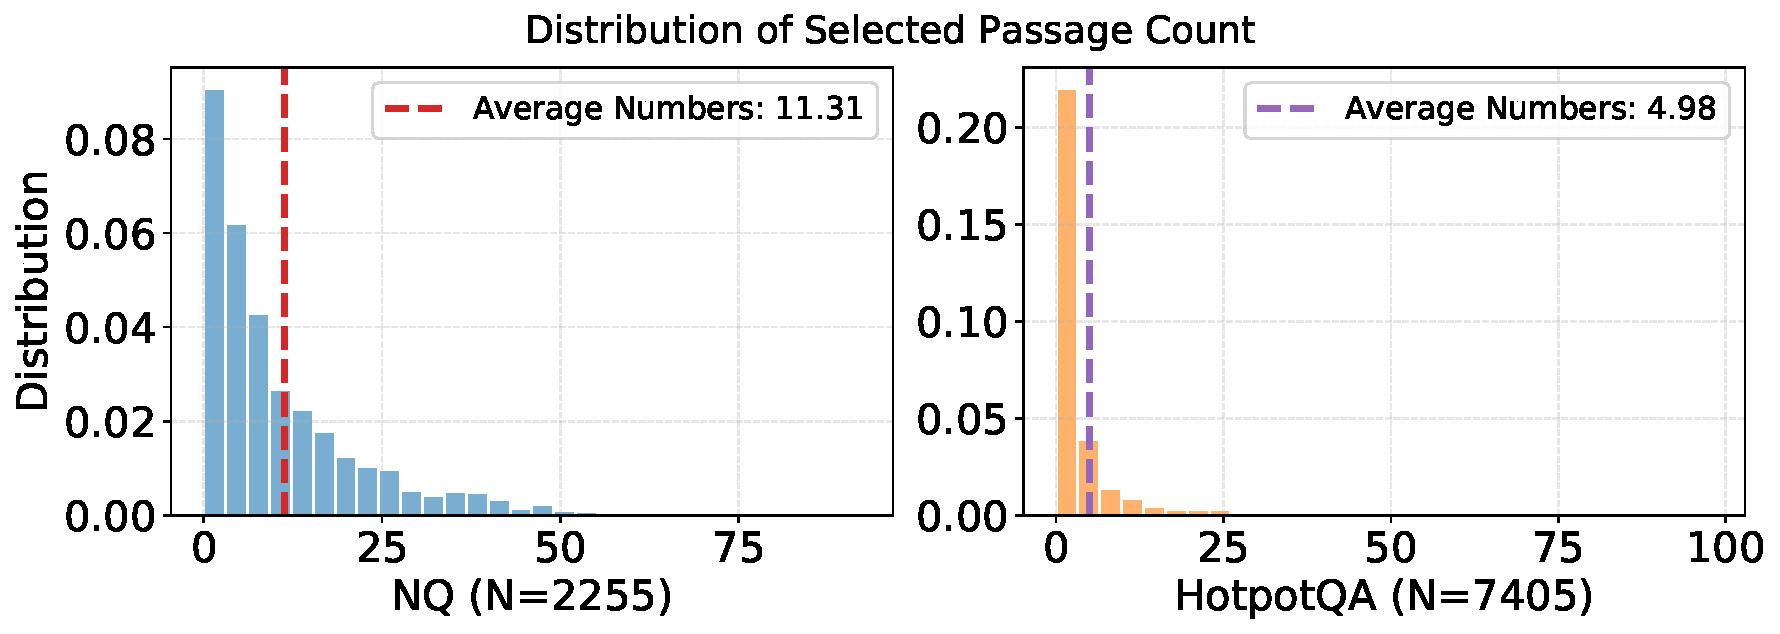
\includegraphics[width=\linewidth]{images/Distribution.pdf}
  \caption{Distribution of selected passage count of \utility$_{1.7B}$ on the NQ and HotpotQA datasets with BM25 retrieval results. ``N'' means the query numbers of the datasets.}
  % \Description{A woman and a girl in white dresses sit in an open car.}
  \label{fig:distribution}
\end{figure}

\begin{figure*}[h]
  \centering
  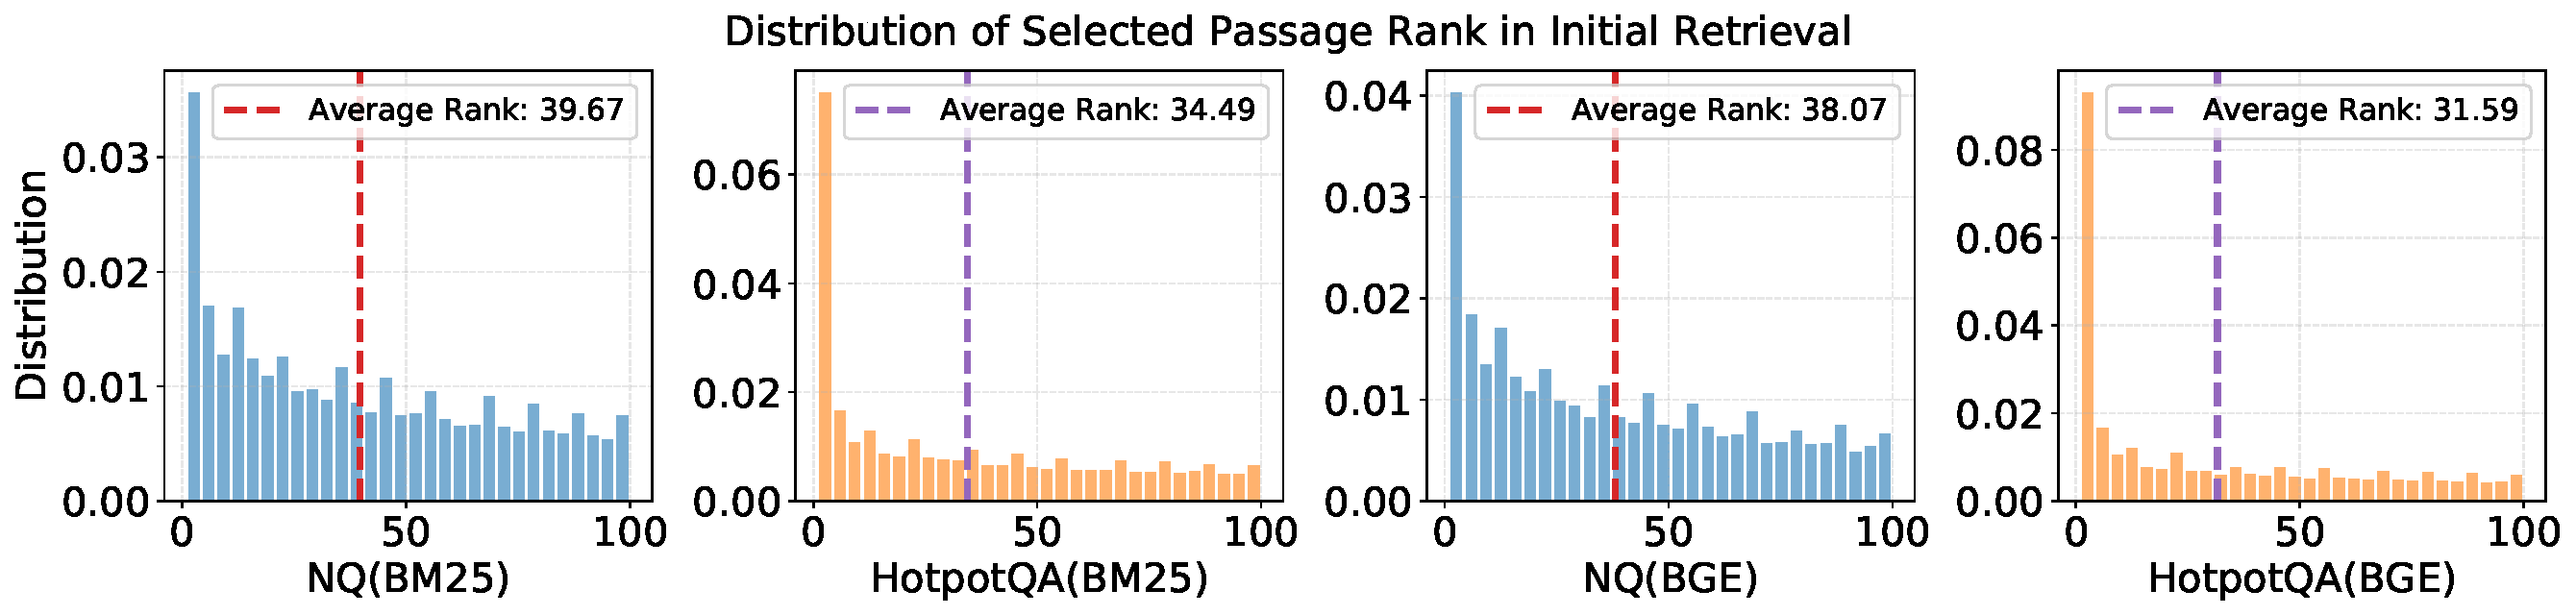
\includegraphics[width=\linewidth]{images/Rank_Distribution.pdf}
  \caption{Distribution of selected passage rank in initial retrieval of \utility$_{1.7B}$ on the NQ and HotpotQA datasets with initial BM25/BGE retrieval results.}
  % \Description{A woman and a girl in white dresses sit in an open car.}
  \label{fig:rank_distribution}
\end{figure*}




\subsection{Impact of LLM Backbone}
To evaluate the performance ceiling of relevance ranking versus utility-based selection in our experimental setup, we directly employed the teacher model (Qwen3-32B) to perform both relevance ranking and utility-based selection on the top-100 BGE-base-en-v1.5 retrieval results for HotpotQA. The selected document sets were then used for downstream answer generation, with results presented in Table \ref{tab:llm_backbone}. Our key observations are: 
1) utility-based selection using the teacher model significantly outperforms threshold-based document selection via relevance ranking in terms of answer generation quality. This further underscores the efficacy of the utility-based approach for evidence selection. 
2) The performance gap between utility-based selection and relevance ranking observed with Qwen3-32B is more pronounced than the corresponding gap between \utility$_{1.7B}$ and \rank$_{1.7B}$. 
This suggests that utility-based selection benefits more substantially from stronger LLM backbones, indicating its greater potential for improvement in RAG applications compared to traditional ranking methods.






\subsection{Statistics of Utility-Based Selection}
Figure \ref{fig:distribution} shows the distribution of passage counts selected as useful by \utility$_{1.7B}$ from the top-100 BM25 results. 
\utility$_{1.7B}$ selects a varying number of useful passages across different queries, with significantly more passages chosen for NQ queries. 


We further analyze the distribution of selected passage ranks from the initial retrieval, as shown in Figure \ref{fig:rank_distribution}. Key observations include:
(1) Our utility-based selection approach retrieves passages across diverse initial ranks, indicating that useful passages may appear at varying positions. This suggests that a fixed threshold may be suboptimal for handling different queries.
(2) The average rank of selected passages is smaller with BGE than with BM25, implying that improved initial ranking (e.g., via BGE) positions utility passages closer to the top. 


% \subsection{Sliding Window for utility-based selection}
\subsection{Inference Efficiency}
% Table generated by Excel2LaTeX from sheet 'Sheet1'
% \begin{table}[htbp]
%   \centering
%   \small
%   \setlength\tabcolsep{3pt}
%   \caption{Analysis of inference efficiency on NQ and HotpotQA datasets with Top-100 BGE retrieval results. ``Avg.win\_num'' represents the average number of windows for each query during the sliding window process. For fair comparison, all the experiments are conducted on eight NVIDIA A800 80GB GPUs.}
%     \begin{tabular}{lllllll}
%     \toprule
%     \multicolumn{1}{c}{\multirow{2}[4]{*}{Method}} & \multicolumn{2}{l}{Avg.win\_num} & \multicolumn{2}{c}{Time} & \multicolumn{2}{c}{RAG(F1)}\\
% \cmidrule(r){2-3} \cmidrule(r){4-5} \cmidrule(r){6-7}    \multicolumn{1}{c}{} & \multicolumn{1}{l}{HotpotQA} & \multicolumn{1}{l}{NQ} & \multicolumn{1}{l}{HotpotQA} & NQ    & \multicolumn{1}{l}{HotpotQA} & \multicolumn{1}{l}{NQ} \\
%     \midrule
%     RankQwen$_{1.7B}$ & 9     & 9    & 11.2h & 3.4h    & 54.25 & 60.17 \\
%     UtilityQwen$_{1.7B}$ & 6     & 7    &   \phantom{1}3.4h    &  1.2h     & 55.73 & 60.95 \\
%     Qwen3-32B (Ranking) &      &     &   &   &  &  \\
%     Qwen3-32B (Selection) &      &     &   &   &  &  \\
%     \bottomrule
%     \end{tabular}%
%   \label{tab:efficiency}%
% \end{table}%


% Table generated by Excel2LaTeX from sheet 'Sheet1'
\begin{table}[t]
  \centering
  \caption{Analysis of inference efficiency on the HotpotQA datasets with Top-100 BGE retrieval results. ``Avg.win\_num'' represents the average number of windows for each query during the sliding window process. For fair comparison, all the experiments are conducted on eight NVIDIA A800 80GB GPUs. The generator is the Llama-3.1-8B-Instruct.}
    \begin{tabular}{lrrr}
    \toprule
    \multicolumn{1}{l}{Method} & Avg.win\_num &  Time & Answer-F1 \\
    \midrule
    Qwen3-32B (Ranking) & 9.0     & 23.3h & 52.03 \\
    Qwen3-32B (Selection) & 6.1   & \phantom{1}6.9h & 59.20 \\
    RankQwen$_{1.7B}$ & 9.0     & 11.2h & 49.68 \\
    UtilityQwen$_{1.7B}$ & 6.4 & \phantom{1}3.4h  & 53.36 \\
    \bottomrule
    \end{tabular}%
 \label{tab:efficiency}%
\end{table}%

Inference efficiency of large language models (LLMs) is a critical practical consideration in RAG deployments. 
Even after distilling the ranking or selection capabilities from a 32B model to a 1.7B model, the inference latency remains significantly higher than that of a 110M cross-encoder model. 
Therefore, we conducted a comparative analysis of the inference efficiency between \rank$_{1.7B}$ and \utility$_{1.7B}$. 
As shown in the Table \ref{tab:efficiency}, we can observe that: 
\begin{enumerate*}
    \item \textbf{Distillation necessity}: Qwen3-32B incurs significantly higher costs than Qwen3-1.7B, underscoring the importance of distillation for practical deployment.  
    \item  \textbf{Efficiency of utility-based selection}: 
    This approach significantly reduces context window consumption and achieves approximately 30\% lower inference latency than relevance ranking.
    Notably, even Qwen3-32B for utility-based selection requires less computational cost than \rank$_{1.7B}$. 
    Furthermore, utility-based selection demonstrates more stable performance compared to the relevance ranking approach. 
\end{enumerate*}


